\documentclass[a0,portrait]{a0poster}

\usepackage{setspace}
\usepackage[scaled]{beramono}
\usepackage[utf8]{inputenc}
\usepackage[tabular,lining]{montserrat}
\renewcommand*\familydefault{\sfdefault}
\usepackage[T1]{fontenc}
\usepackage[portuges]{babel}
\usepackage{amsfonts, amsmath, amsthm, amssymb}
\usepackage{graphicx, url, float, booktabs, datetime, multicol}
\usepackage{lipsum, cite, wrapfig}
\usepackage[hang]{subfig}
\usepackage[font=large,labelfont=bf]{caption}
\usepackage[ruled]{algorithm2e}
\usepackage[super]{nth}
\usepackage[hang]{subfig}
\usepackage[svgnames]{xcolor} % Specify colors by their 'svgnames', for a full list of all colors available see here: http://www.latextemplates.com/svgnames-colors
\usepackage[
    breaklinks=true,    
    allbordercolors=Indigo,
%    ocgcolorlinks=true,
    colorlinks=true,
    anchorcolor=Indigo, 
    citecolor=black,
    filecolor=Indigo,
    linkcolor=Indigo,
    menucolor=Indigo,
    runcolor=Indigo,
    urlcolor=Indigo,
    linktoc=all
]{hyperref}
\usepackage[ocgcolorlinks]{ocgx2}

\usepackage{pgf}
\usepackage{pgfpages}

\pgfpagesdeclarelayout{boxed}
{
  \edef\pgfpageoptionborder{0pt}
}
{
  \pgfpagesphysicalpageoptions
  {%
    logical pages=1,%
  }
  \pgfpageslogicalpageoptions{1}
  {
      border code=\pgfsetlinewidth{4pt}\color{Indigo}\pgfstroke,%
    border shrink=\pgfpageoptionborder,%
    resized width=.95\pgfphysicalwidth,%
    resized height=.95\pgfphysicalheight,%
    center=\pgfpoint{.5\pgfphysicalwidth}{.5\pgfphysicalheight}%
  }%
}

\pgfpagesuselayout{boxed}

\columnsep=100pt
\columnseprule=4pt

\usepackage{sectsty}
\usepackage[most]{tcolorbox}

\tcbset{
    frame code={}
    center title,
    left=0pt,
    right=0pt,
    top=0pt,
    bottom=0pt,
    colback=Indigo!10,
    colframe=black,
    width=\dimexpr\linewidth\relax,
    enlarge left by=0mm,
    boxsep=3pt,
    arc=0pt,outer arc=0pt,
    }

\usepackage{tikz}
    \usetikzlibrary{positioning}
    \usetikzlibrary{arrows}

\tikzset{basic/.style={draw,fill=Gray!50,text width=1em,text badly centered}}
\tikzset{input/.style={basic,circle}}
\tikzset{weights/.style={basic,rectangle}}
\tikzset{functions/.style={basic,circle,fill=Gray!25}}
\tikzset{int/.style={draw, fill=Gray!50, minimum size=2em}}

% \allsectionfont{\fontfamily{Montserrat-TOsF}}

\setlength\parindent{5cm}

\begin{document}

    \noindent
\begin{minipage}{0.73\linewidth}
    % \headingfont
\veryHuge \color{Indigo} \textbf{Fundamentos de Redes Neurais Profundas:}\\ \color{Black}
\LARGE\textit{Abordagem Baseada em Redes Convolucionais.}\\[1cm] % Subtitle
\LARGE \textbf{Rafael Gonçalves \& Romis Attux.}\\[0.2cm] % Author(s)
    {\LARGE Faculdade de Engenharia Elétrica e de Computação - Unicamp\\
    \texttt{r186062@dac.unicamp.br, attux@dca.fee.unicamp.br}}
\end{minipage}
%
\begin{minipage}{0.27\linewidth}
    \centering
    \vspace{2cm}
    \def\svgwidth{0.6\columnwidth}
    \input{unicamp.pdf_tex}
    \break\hfill\break
\end{minipage}

\vspace{1cm} % A bit of extra whitespace between the header and poster content

\begin{multicols}{2}

% \onehalfspacing
    \section*{\begin{tcolorbox}
        \LARGE
        % \headingfont
        \centering
        Introdução
    \end{tcolorbox}}

\large

    Redes neurais artificiais são sistemas de computação não lineares e adaptativos originalmente inspirados nas redes neurais biológicas presentes no sistema nervoso dos animais.
    Especialmente com o advento de redes neurais profundas e o conceito de aprendizado profundo, este se tornou um importante paradigma dentro do campo de aprendizado de máquina e é amplamente utilizado para resolver uma variedade de problemas atuais.

    Neste contexto, esta pesquisa buscou estudar teoricamente redes neurais profundas baseado em um livro recente e representativo ~\cite{Goodfellow16} e posteriormente aplicar um modelo específico de rede neural -- a saber uma rede convolucional -- ao problema conhecido de reconhecimento de dígitos escritos à mão utilizando a base de dados MNIST ~\cite{mnist}.

    \section*{\begin{tcolorbox}
        \LARGE
        % \headingfont
        \centering
        Discussões e Resultados
    \end{tcolorbox}}
    \large

    \subsection*{\Large\color{Indigo}Perceptron de Múltiplas Camadas -- MLP}

As redes MLP podem ser vistas como redes de neurônios perceptron interligados em forma de camadas: uma camada de entrada que recebe cada entrada do vetor $\mathbf{x}$, uma ou mais camadas intermediárias e uma camada de saída. Exemplo de uma rede MLP pode ser visto na figura ~\ref{fig:mlp}.

  \begin{figure}[H]
        {\centering
        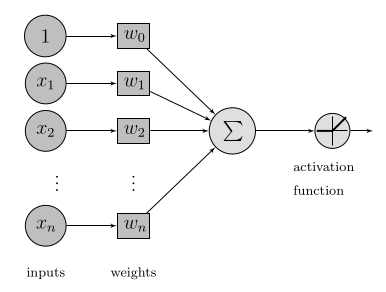
\includegraphics[width=.4\linewidth]{neuron.png}
        \caption{Neurônio de tipo perceptron.}
        \label{fig:mlp}\par}
  \end{figure}

    Desta forma, matematicamente a saída de uma dessas redes -- considerando $\mathbf{w^n}$, $w_0^n$ e $f^n$ como respectivamente matriz de pesos, viés (\em bias\em ) e função de ativação da camada n --  é:

    \begin{equation}
  y = f^N(\mathbf{w^N}\cdot ... f^2(\mathbf{w^2}\cdot f^1(\mathbf{w^1} \cdot \mathbf{x} + w_0^1) + w_0^2) + w_0^N)
    \end{equation}


    Ou ainda, se definirmos uma matriz de entrada que admita $M$ exemplos em uma mesma estrutura -- podemos ainda definir um vetor $\mathbf{W}$ que inclua $w_0$ no vetor $\mathbf{w}$ e definir uma matriz $\mathbf{\Phi}$ cuja linha $\mathbf{\phi_{i}} = [1 \quad \mathbf{x_i}]$ com $i$ indicando cada exemplo:

\begin{equation}
    \label{eq:mlp}
  \mathbf{y} = \mathbf{F^n}( ... \mathbf{F^2}(\mathbf{F^1}(\boldsymbol{\Phi} \cdot \mathbf{W^1})\mathbf{W^2})\mathbf{W^N})
\end{equation}

%   Com:
% \break\hfill\break
% $
% \boldsymbol{\Phi} = \begin{bmatrix}
%     1 & \mathbf{x_1} \\
%     1 & \mathbf{x_2} \\
%     &\vdots \\
%     1 & \mathbf{x_M}
% \end{bmatrix}
% $
% \hfill
% $
% \mathbf{y} =\begin{bmatrix}
%     y_1 \\
%     y_2 \\
%     \vdots \\
%     y_M
% \end{bmatrix}
% $
% \hfill
% $
% \mathbf{{F^n}(u)} = 
% \begin{bmatrix}
%   f^n(u_1) & 0 & \cdots  & 0 \\
%   0 & f^n(u_2) & \cdots  & 0 \\
%   \vdots   & \vdots & \ddots & \vdots \\
%   0 & 0 & \cdots  & f^n(u_M) \\
% \end{bmatrix}
% $

  \begin{figure}[H]
        {\centering
        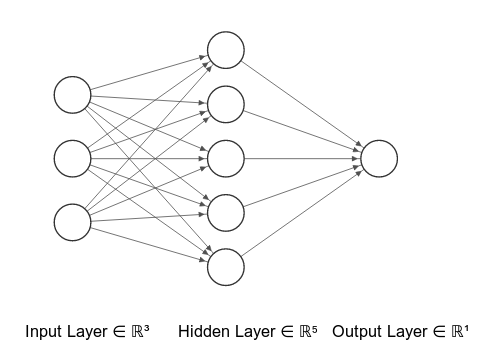
\includegraphics[width=.45\linewidth]{mlp_ex.png}
        \caption{Exemplo de rede MLP com 3 atributos de entrada, uma camada intermediária com 5 neurônios e uma camada de saída com um único neurônio, gerado com ~\cite{nnsvg}.}
        \label{fig:mlp}\par}
  \end{figure}

    \subsection*{\Large\color{Indigo}Rede Neural Convolucional -- CNN}

 Redes CNN são arquiteturas de ANNs com ao menos uma camada convolucional. Camadas convolucionais usam kernels de pesos e a operação matemática de convolução para gerar a informação de saı́da do neurônio, diferentemente das MLPs que usam o produto interno da entrada com um vetor de pesos.

  Exemplo da operação de convolução entre uma imagem $\mathbf{I}$ 2D e um kernel $\mathbf{K}$:

\begin{equation}
  (I*K)(i, j) = (K*I)(i,j) = \sum_m\sum_n K(m, n) \cdot I(i-m, j-n)
\end{equation}

% \begin{figure}[H]
%     {\centering
%     \begin{tikzpicture}[node distance=10em,auto,>=latex']
%         \node [int] (a) {Convolution};
%         \node [int] (c) [right of=a] {Activation};
%         \node [int] (e) [right of=c] {Pooling};
%         \path[draw,->] (a) -- (c);
%         \path[draw,->] (c) -- (e);
%     \end{tikzpicture}
%     \caption{Etapas de uma camada convolucional.}
%     \label{fig:conv}\par}
% \end{figure}

  \begin{figure}[H]
        {\centering
        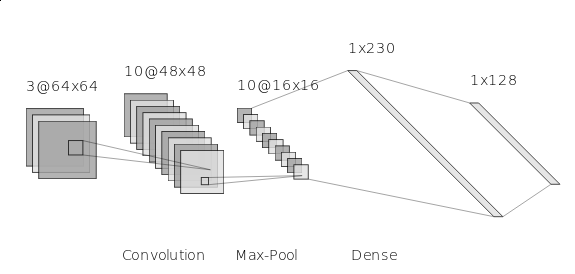
\includegraphics[width=.6\linewidth]{cnn_ex.png}
        \caption{Exemplo de rede CNN com 1 camada convolucional - convolução e max-polling - e 2 camadas FC, gerado com ~\cite{nnsvg}.}
        \label{fig:cnn}\par}
  \end{figure}

  Redes MLP e CNN foram implementadas com diferentes configurações para dropout (no caso de ambas as arquiteturas) e quantidade de neurônios nas camadas internas (na arquitetura MLP).

  \begin{figure}[H]
        {\centering
        \break\hfill\break
        \break\hfill\break
        \color{Indigo}
        \textbf{\large Progressão do erro ao longo das épocas de treinamento.}\par\medskip
        \subfloat[Modelo MLP.]{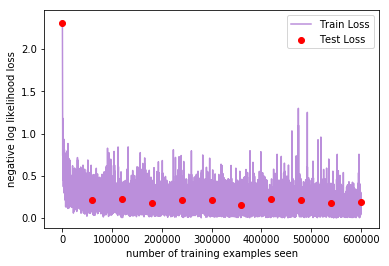
\includegraphics[width=.5\linewidth]{mlp.png}}
        \hfill
        \subfloat[Modelo CNN.]{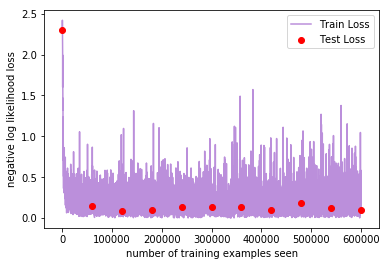
\includegraphics[width=.5\linewidth]{cnn.png}}
        \caption{Curva de aprendizado dos melhores modelos de cada tipo de arquitetura.}
        \label{fig:lc}\par}
  \end{figure}

O resultado final dos melhores modelos estão na tabela ~\cite{tab:final}.

\vspace{1em}

\begin{table}[H]
\caption{Modelos finais avaliados no conjunto de teste.}
\centering
    \label{tab:final}
\large
% \begin{tabular}{@{}lll@{}}
% \toprule
%     Modelo \fill & Melhor Época  & \hfill Melhor Acurácia \\ \midrule
%     MLP  &         10  & 0.9663   \\
%     CNN  &          7  & 0.9771   \\ \bottomrule
% \end{tabular}
% \end{table}

\begin{tabular}{||c|c|c||}
    \hline
    Modelo \fill & Melhor Época  & \hfill Melhor Acurácia \\ \midrule
    \hline\hline
    MLP  &         10  & 0.9663   \\
    \hline
    CNN  &          7  & 0.9771   \\
    \hline
\end{tabular}
\end{table}
    
    \section*{\begin{tcolorbox}
        \LARGE
        % \headingfont
        \centering
        Conclusões
    \end{tcolorbox}}
    \large

    O estudo mostrou que tanto a arquitetura MLP como a CNN são viáveis para o problema de classificação de dígitos escritos a mão ~\cite{mnist}. O modelo final de rede convolucional apresentou um resultado ligeiramente melhor -- acurácia de 97.8\% em comparação à 96.7\% referente à MLP.

    O uso de dropout teve pouca influência em ambas as arquiteturas, sendo que nas redes MLP o mesmo contribuiu negativamente para o aumento da acurácia e nas redes CNN um dropout de 30\% foi o que proveu o maior índice. Nas redes MLP a variação do número de neurônios nas camadas intermediárias teve pouca influência o problema pode ser resolvido por modelos mais simples.

    
    \section*{\begin{tcolorbox}
        \LARGE
        % \headingfont
        \centering
        Agradecimentos
    \end{tcolorbox}}
    \large

    O estudante gostaria de expressar seu agradecimento ao programa PIBIC/CNPq/Unicamp pelo auxílio financeiro e em especial à Romis Attux por todo o incentivo e apoio durante o desenvolvimento da pesquisa.

    

    \noindent
    \rule{.33\linewidth}{2pt}

{\normalsize
\begin{thebibliography}{9}
    \bibitem{Goodfellow16}
        I. Goodfellow, Y. Bengio, A. Courville.
        \textit{Deep Learning}.
        MIT Press, 2016.
    \bibitem{mnist}
        Y. LeCun.
        \textit{The MNIST Database of Handwritten Digits}.
        \url{http://yann.lecun.com/exdb/mnist}.
        (acessado em 07/07/2019).
    \bibitem{github}
        R. Gonçalves.
        \textit{mnist\_nn}.
        \url{https://github.com/RafaelGoncalves8/mnist_nn}
        (acessado em 20/07/2019).
    \bibitem{nnsvg}
        LeNail.
        \textit{NN-SVG: Publication-Ready Neural Network Architecture Schematics}.
        \url{http://alexlenail.me/NN-SVG/}.
        Journal of Open Source Software, 2019.
        (acessado em 20/07/2019).
\end{thebibliography}
}
\end{multicols}

\end{document}
